%% Basic documentation
%%
%% (c) Thomas Hesse
%%
%% folder: ./content/

\chapter{Introduction}
\label{chap:0}
%
% TODO remove this guide and start writing your thesis :-)
%
\section{Getting~started}
%
	\subsection{Installing~Glossaries}
		\bf{Note for Windows users:} While the makeglossaries command is a perl script for Unix users, there is also a .bat version of the file for Windows users. However, I don’t know how to set up MIKTex or equivalent to use this package. Feel free to add a comment if you can add information about this step.

		\begin{enumerate}
	%
	% 1
			\item \bf{Get and unzip the glossaries package.} I downloaded it from \href{http://www.tex.ac.uk/tex-archive/install/macros/latex/contrib/glossaries.tds.zip}{here}. Though you can download the source and compile, I found it much easier to simply download the tex directory structure (tds) zip file.  Unfortunately, the texlive-latex-extra package available on ubuntu or kubuntu does not contain the glossaries package – it only contains glossary and acronym. I unzipped the contents of the zip file into a directory called “texmf” in my home directory. You’ll also want to run “texhash ~/texmf/” to update the latex database, according to the INSTALL instructions. %
	%
	% 2
			\item \bf{(Optionally) get the xfor package.} If your system is like mine, after you’ve installed the glossaries package latex will complain that it doesn’t have the xfor package (which also is not available via apt-get in Ubuntu). Download this package from \href{http://tug.ctan.org/tex-archive/macros/latex/contrib/xfor/}{here}. %
	%
	% 3
			\item \bf{Open the glossaries zip \ul{as root} in a nautilus window, terminal window, or equivalent.} You’ll be copying the contents to various locations in the root directory structure, and will need root access to do this. %
	%
	% 4
			\item \bf{Find the location of your root texmf directory.} In Karmic, this is /usr/share/texmf/, though it may be in another location on your system. Generally, you should have a local texmf folder, i.e. ~/texmf/, when receiving the IAS slide \LaTeX~template. %
	%
	% 5
			\item \bf{Copy the contents of the tex and doc directories from the glossaries zip into the matching directory structure in your texmf directory.} For me, this meant copying the “doc/latex/glossaries” subdirectory in the zip file to “/usr/share/texmf/doc/latex/”, and the same for the tex directory (copy “tex/latex/glossaries” subdirectory in the zip file to “/usr/share/texmf/tex/latex/”). In theory, you can also copy the scripts/ directory in the same way, but I did step 6 instead, as this is what was suggested in the INSTALL document.
	%
	% 6
			\item \bf{Update the master latex database.} Simply run the command “sudo mktexlsr”
	%
	% 7
			\item \bf{Add the location of your scripts/glossaries directory to your \$PATH.} This gives programs access to makeglossaries, the perl script you will be using (if you’re in linux/unix). If you followed my default instructions in step 1, this location will be “/home/yourname/texmf/scripts/glossaries”.
	%
	% 8
			\item \bf{Test the installation.} Change into the directory you created in step 1, into the “doc/latex/glossaries/samples/” subdirectory. There, run “latex minimalgls”. If you get an error about xfor, please see step 9. Otherwise, run “makeglossaries” and then “latex minimalgls” again. If everything works, the package is set up for command-line use. You may wish to modify your Kile setup to use glossaries – go to step 10 if this is the case.
	%
	% 9
			\item \bf{Set up the xfor package.} Run steps 3-6 again, but with the xfor.tds.zip file instead of the glossaries zip file. This package is simpler than glossaries, and does not contain a scripts/ subdirectory, so you will not need to do step 7. After installation, try running step 8 again: everything should work.
		\end{enumerate}
		\mbox{\bf{Source:} \href{http://themindwobbles.wordpress.com/2009/12/16/using-the-glossaries-package-in-latex-and-linux-kile/}{link}}
%
%
%

	\subsection{Configure the Modification of the TU Design}
	You can find in the IAS Thesis folder a folder with the name \textit{texmf}. 			This folder includes some modifications of the TUD design, for example an updated Thesis statement in english and german.
	After the installation of the TUD design (\url{http://exp1.fkp.physik.tu-darmstadt.de/tuddesign/}) you have to move the folder to your home folder. If the folder already exists, then move only the tud-files.
	Then you have to run the command \textit{texhash $\sim$/texmf } such that Latex can use the new files.
	Please note, that the texmf folder already includes some adaptions for the tud-beamer template. If you want to use the original TUD design again, rename the texmf folder and run texhash again.
	
	If you have questions regarding the modifications of the TU design or suggestions, please let me know and send me an email to luck@ias.tu-darmstadt.de
\newpage
\section{Documentation}
%
	\subsection{Structure~of~the~IAS~\LaTeX-Framework}
		The structure of this framework is illustrated in the following figure. %
		\begin{figure}[H]
			\centering
			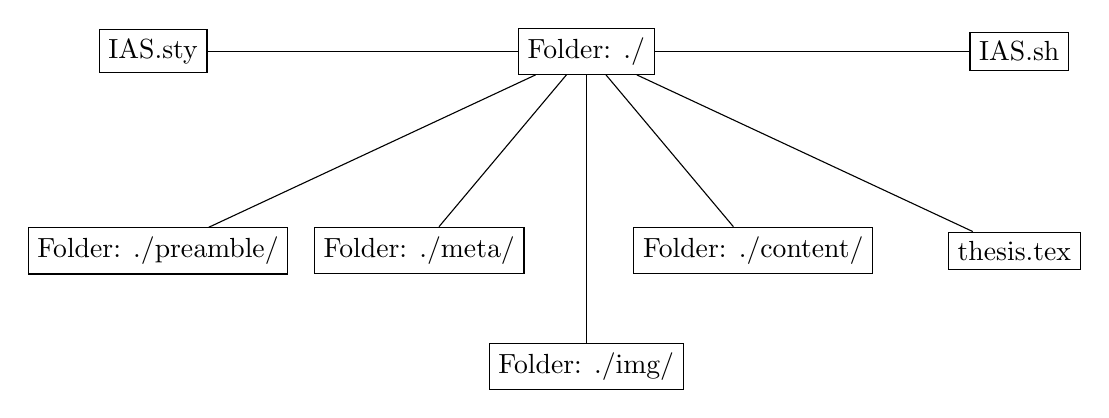
\begin{tikzpicture}[
			    node/.style={%
			      draw,
			      rectangle,
			    },
			  ]
			    \node [node] (root) {Folder: ./};
			    \path (root) ++(-25:60mm) node [node] (thesisTex) {thesis.tex};
			    \path (root) ++(0:55mm) node [node] (IASSH) {IAS.sh};
			    \path (root) ++(180:55mm) node [node] (IASSTY) {IAS.sty};
			    \path (root) ++(-50:33mm) node [node] (content) {Folder: ./content/};
			    \path (root) ++(-130:33mm) node [node] (meta) {Folder: ./meta/};
			    \path (root) ++(-155:60mm) node [node] (preamble) {Folder: ./preamble/};
			    \path (root) ++(-90:40mm) node [node] (img) {Folder: ./img/};
			    \draw (root) -- (IASSTY) node [below,midway] {}(root);
			    \draw (root) -- (IASSH) node [below,midway] {}(root);
			    \draw (root) -- (thesisTex) node [below,midway] {}(root);
			    \draw (root) -- (content) node [above,midway] {}(root);
			    \draw (root) -- (meta) node [above,midway] {}(root);
			    \draw (root) -- (preamble) node [below,midway] {}(root);
			    \draw (root) -- (img) node [below,midway] {}(root);
			\end{tikzpicture}
			\label{fig:structure}
			\caption{The structure of the IAS~Thesis~\LaTeX-Framework illustrated.}
		\end{figure}
		The \bf{./preamble/} folder should contain content that needs to be processed in the preamble section, i.e. before \texttt{\bs{}begin\{document\}}, as the name suggests. %
		\\[0.2cm]%
		The \bf{./meta/} folder should contain content that is not directly related to the topic of the thesis or summarizes content of the thesis, i.e. \texttt{abstract.tex} or \texttt{acknowledgements.tex}. %
		\\[0.2cm]%
		The \bf{./img/} folder should solely contain images, e.g. \texttt{png}, \texttt{eps}, etc. %
		\\[0.2cm]%
		The \bf{./content/} folder is the most important for the user eversince you stuff in all your content related files / chapters in here. %
		You can \texttt{\bs{}input\{yourFile\}} afterwards in the \texttt{./thesis.tex} where the content variable is defined. %
	%
	%
	%
	\subsection{Commands~\&~shortcuts}
		There are several shortcuts and commands you should memorize! %
		\begin{itemize}
			\item Wrapper command for vectors\begin{verbatim} \cvec{} \end{verbatim} Example: $\cvec{v}$
			\item Wrapper command for matrices\begin{verbatim} \cmat{} \end{verbatim} Example: $\cmat{M}$
			\item Shortcut for \texttt{\bs{}textbf\{\}}\begin{verbatim} \bf{} \end{verbatim} Example: \bf{bold font}
			\item Shortcut for \texttt{\bs{}textit\{\}}\begin{verbatim} \it{} \end{verbatim} Example: \it{italic font}
			\item Shortcut for \texttt{\bs{}underline\{\}}\begin{verbatim} \ul{} \end{verbatim} Example: \ul{underline}
			\item Shortcut for \texttt{\bs{}mathcal\{\}}\begin{verbatim} \mc{} \end{verbatim} Example: $\mc{N}(\mu,\Sigma)$
		\end{itemize}
	%
	%
	%
	\subsection{Getting~started~with~Glossaries}
		For a comprehensive guide to glossaries, you should read \href{http://en.wikibooks.org/wiki/LaTeX/Glossary}{this article}. %
		There is also sample code given in \texttt{./preamble/glossary.tex} which you should have a look at as well!